\chapter{\ucosiii on the Raspberry Pi}
Real-time operating systems run on a broad range of hardware. Running tests on all of this different hardware is, of course, impossible. For this thesis, I have chosen to use a piece of hardware which exemplifies a number of characteristics of real-time systems, but which is also readily available and well-documented: a first-generation Raspberry Pi.

\section{The Raspberry Pi 1B}
The hardware used in this thesis is a Raspberry Pi 1B, a single-board computer from early 2012. While it was marketed as an educational `toy' for children to learn how to program on, it became popular mainly as a cheap development board for (hardware) hobbyists, due to its ability to control electronics using its general purpose I/O (GPIO) pins, and its low price point of \$25-35 (depending on model). Its hardware is as follows:

\begin{outline}
    \1 A Broadcom BCM2835 System-on-Chip, including:
        \2 A single-core 700MHz ARM11 (ARMv6) processor
        \2 A VideoCore IV graphics processor
        \2 512 megabytes of RAM
    \1 26-pin General Purpose I/O (GPIO) header, capable of performing various functions
        \2 Serial I/O, SPI, software-controlled reading and writing at 3.3V
    \1 Ethernet, USB, HDMI and composite out, et cetera.
\end{outline}

The Pi has a number of desirable characteristics that make it suitable for use in this thesis. Firstly, it uses a low-power ARM processor, an architecture which is very common in embedded systems (with a market share of 37\% at the end of 2014 \cite{arm:embeddedmarketshare}). Additionally, its GPIO pins and their support for serial I/O allow for a simple way of interacting with the Raspberry Pi without having to implement USB or Ethernet drivers. Such serial connections are also very common in embedded systems. Lastly, due to the popularity of the Pi, it is fairly well-documented. The datasheet that describes the hardware in the Raspberry Pi and how to interface with it is freely available\cite{bcm:2835peripherals}, and although it is occasionally inaccurate, there is a thorough list of errata available online\cite{bcm:2835errata}. Where the datasheet has omissions, there is also often information available online.

\section{The structure of \ucosiii}
The majority of \ucosiii is written as processor-independent C code, and can therefore be re-used in the port verbatim. Fragments of the operating system whose implementation is highly dependent on the target hardware, such as task switching or interaction with hardware timers, are implemented in separate source files. There is a CPU-specific component, \ucpu, which specifies CPU features such as the availability of a count-leading-zeros instruction, endianness, the size of data types such as timestamps, addresses, et cetera. Separately, OS-specific components such as task switching functions are defined. Lastly, a `Board Support Package' is defined, which contains the functionality that interacts with the on-board components such as the hardware timer and handles interrupts.

\section{Porting \ucosiii to the Raspberry Pi}
To run \ucosiii on the Raspberry Pi, the operating system needs to be adapted to run on the hardware the Pi uses. These adaptations are commonly called \textit{ports}. There are ports to architectures that are similar to that of the Pi, such as the ARM9-based NXP LPC2923 \cite{micrium:nxplpc}, but there is no port for the Broadcom BCM2835, the SoC used by the Pi. This work includes such a port. Below, various parts of the port and the ways they hook into the Raspberry Pi's hardware are discussed.

\subsection{Bootup}
The Raspberry Pi's startup process is largely handled by the VideoCore IV GPU, which runs a real-time operating of its own, ThreadX, and aside from being a graphics accelerator handles `embedded controller' tasks such as clock and power management. The boot process, as described in \textcite{rpi:bootforum}, is roughly as follows. The first-stage bootloader is programmed into ROM when the Raspberry Pi is manufactured, and it loads the second-stage bootloader \code{bootcode.bin} from the first SD card partition. \code{bootcode.bin} loads the GPU firmware, \code{start.elf}, which initializes hardware and sets up memory based on parameters in \code{config.txt}, loads the kernel (by default \code{kernel.img}) to address \code{0x8000}, and releases the ARM CPU from reset.

To reduce the amount of work when updating the kernel, the port includes a serial bootloader, which replaces the \code{kernel.img} file on the SD card, and when executed relocates itself high into memory before loading the kernel over the serial connection and executing it. This way, running a new version of the kernel was as simple as unplugging and replugging the USB power cable and running the \code{run} script on the host.

After the kernel is loaded, the port startup code (\code{startup.s}) configures and initializes the processor, by setting up stack pointers, initializing interrupt vectors and enabling the floating-point unit, branch predictor, and instruction cache\footnote{Data cache cannot be enabled without using virtual memory, as it would interfere with memory-mapped peripherals. It is left disabled in the interest of time.}. After initializing the C environment by zeroing out the BSS, control is transferred to the C main function. In C, hardware such as serial I/O ports and the timer interrupt are configured using functions in the board support package. Lastly, the OS is initialized with the \code{OSInit} function, tasks are created, and the operating system is started with the \code{OSStart} function.

\subsection{Timers}
In real-time systems, there obviously needs to be a correspondence between the time as measured in the system and external time. This is where hardware timers come in. The Raspberry Pi provides both running counter functionality (which allows the system to have a clock -- though it is not a real-time clock, which would keep an accurate date and time of day across reboots) and timer functionality (so the system is interrupted after a given time is elapsed).

As described in the BCM2835 peripheral data sheet, the Raspberry Pi contains two timers; a timer for the ARM processor itself and a system timer. Although \textcite{sfd:realpi} opts to use the ARM timer, the peripheral data sheet suggests using the system timer when accurate timing is required.\cite[p. 196]{bcm:2835peripherals}.

The system timer has microsecond resolution\footnote{Although the ARM timer has a higher frequency, it is not useful to us as the time taken to switch between tasks is already in the microsecond range.}, and consists of a 64-bit running counter and four 32-bit timer channels. These timer channels have a corresponding match register, which contains a 32-bit value that is compared with the running counter, triggering an interrupt when the lowest 32 bits of the running counter match the register value.

Two of the timer channels are in use by the VideoCore IV GPU, and are therefore not usable. Timer channel 1 and 3 are, however, available. We only need a single timer channel, and currently use timer channel 1.

\subsection{Interrupts}
As discussed in the previous section, the hardware timer can trigger an interrupt when a timer channel is matched. The system timer is one of the hardware components which is poorly described in the peripheral data sheet, but information found online can close that gap.

Interrupt handling in the ARM architecture differs significantly from similar features in the x86 architecture. Where the latter uses an interrupt vector table which dispatches a specific interrupt to a specific interrupt service routine, the former uses a much more generic approach.

ARM uses the term `exception' to mean an event which causes the processor to stop execution and jump to a piece of code to handle it. The ARM architecture supports seven kinds of exceptions: \textit{Reset}, \textit{Undefined Instruction}, \textit{Software Interrupt}, \textit{Prefetch Abort}, \textit{Data Abort}, \textit{Interrupt} (IRQ) and \textit{Fast Interrupt} (FIQ). When an exception is generated, the CPU jumps to an \textit{exception vector} for the given exception. These vectors are usually located at the beginning of the address space, but can be remapped. An overview of exception types, their corresponding processor mode and address that execution starts at after exception reception is given in table~\ref{tbl:exceptions}.

\begin{table}[h]
    \centering
    \begin{tabular}{lll}
        \toprule
        \textbf{Exception type} & \textbf{Processor mode} & \textbf{Execution address} \\
        \midrule
        Reset & Supervisor & \texttt{0x00000000} \\
        Undefined instructions & Undefined & \texttt{0x00000004} \\
        Software interrupt & Supervisor & \texttt{0x00000008} \\
        Prefetch Abort & Abort & \texttt{0x0000000C} \\
        Data Abort & Abort & \texttt{0x00000010} \\
        IRQ (interrupt) & IRQ & \texttt{0x00000018} \\
        FIQ (fast interrupt) & FIQ & \texttt{0x0000001C} \\
        \bottomrule
    \end{tabular}
    \caption{An overview of ARM exceptions. Adapted from table A2-4 in the ARM Architecture Reference Manual\cite{arm:arm}.}
    \label{tbl:exceptions}
\end{table}

In effect, processor faults and software interrupts have their own exception, and all `normal' device interrupts are coalesced into the `interrupt' and `fast interrupt' exceptions. The exception handling code, then, is tasked with determining which device caused the interrupt. The means of determining the interrupting device differ, as they often rely on hardware-provided memory-mapped registers. This is no different on the Raspberry Pi -- the peripheral data sheet details the interrupt mechanism in some detail on page 109. The peripheral data sheet however fails to mention the interrupt number assigned to the system timer. Some sleuthing reveals that the system timer channels are mapped at the start of the interrupt numbers, so IRQ 0 refers to the first timer channel, IRQ 1 to the second, et cetera.

As mentioned, the interrupts are handled either by the `fast interrupt' handler or the normal `interrupt' handler. The BCM2835 allows the systems programmer to route a single interrupt source to the fast interrupt vector, which has more banked registers and therefore allows for faster interrupt processing. This is not used in the port currently, as it would complicate the task switching code, which can currently use the same assembly for returning to voluntarily yielded code and interrupted code.

\subsection{General Purpose I/O}
The Raspberry Pi has 26 general purpose I/O pins. Some of these pins have a fixed function, but many have multiple functions, and which one a pin uses can be controlled by software. An overview of the 26-pin header and the functions of its pins can be seen in figure~\ref{fig:gpiopinout}. One thing of note is the fact that the pin numbering used on the header is not the same as is used in the BCM2835 peripherals manual; for instance, pin 7 on the header is GPIO pin 4 in the data sheet.

\begin{figure}[ht]
    \centering
    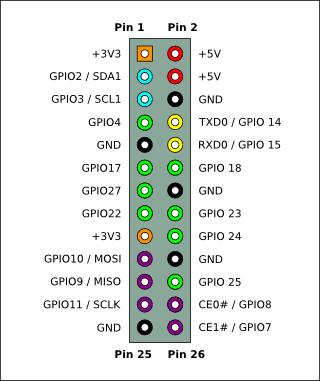
\includegraphics[scale=0.5]{figures/Pi-GPIO-header-26-sm.png}
    \caption{The Raspberry Pi 1B GPIO pinout. Pins labeled \textit{GPIO \#} correspond to GPIO pins in the Broadcom BCM2835 peripherals manual\cite{bcm:2835peripherals}.}
    \label{fig:gpiopinout}
\end{figure}


\subsection{Serial I/O} \label{sec:miniuart}
Implementing input/output capabilities is not strictly required to get \ucosiii running on the Raspberry Pi. An operating system is of little use without any I/O capabilities, however, and being able to output debugging information is also of great use in porting.

The type of I/O that the port has support for is very common in embedded devices, and was used throughout much of the twentieth century for communication between computers and associated terminals: serial communication using a UART. The peripheral data sheet tells us that the Raspberry Pi contains two UARTs, a primary ARM PL011 UART and a secondary so-called `mini UART'. Due to limitations such as the shallow FIFOs, this port uses the primary UART.

On the hardware side, the UART uses GPIO pins 8 and 10\footnote{Pin 14 and 15, respectively, in the Broadcom peripheral datasheet.} for transmit and receive, respectively. Additionally, one of the Pi's ground pins needs to be used to ensure the communicating devices have a common ground.

%\subsection{Hardware watchdog}
